
\begin{figure}
	
 \centering
    \begin{minipage}{0.49\textwidth}
   
        \centering
        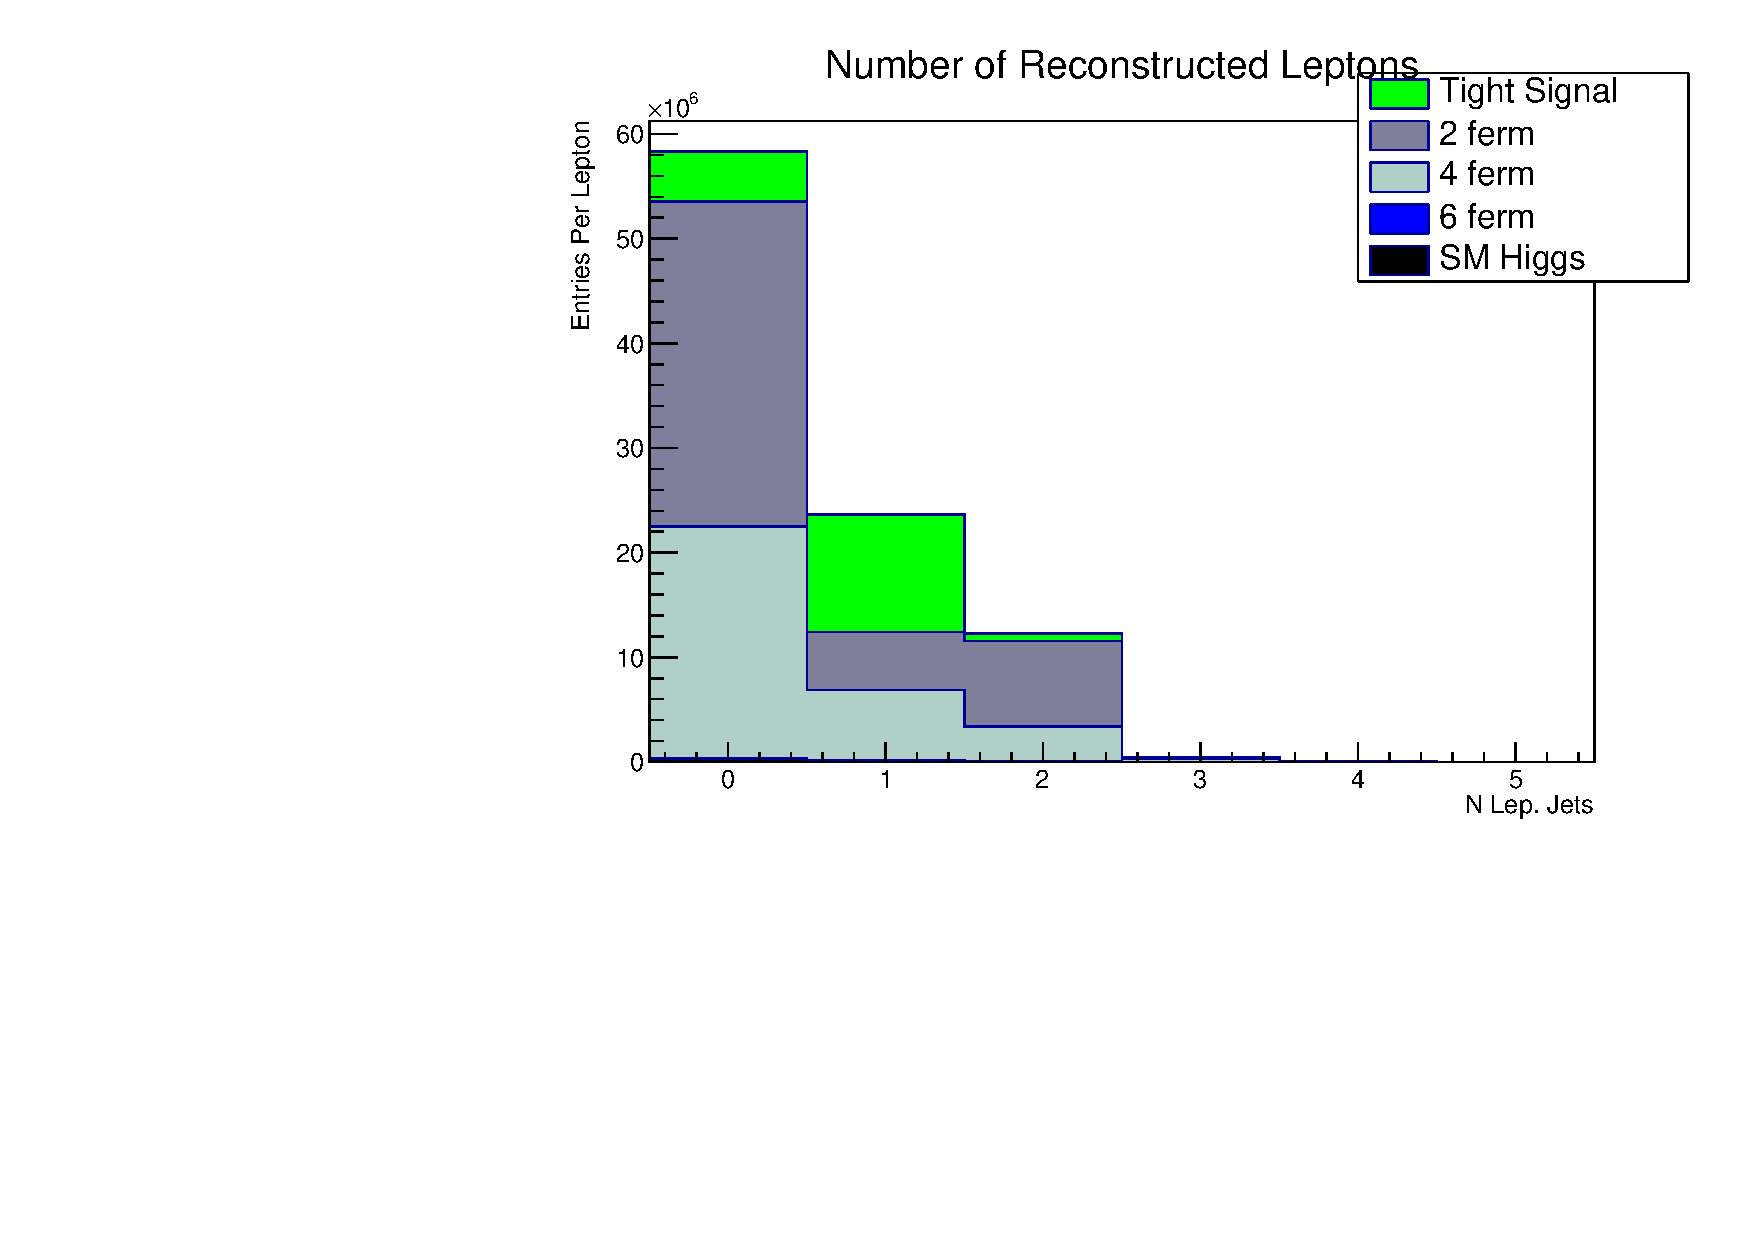
\includegraphics[width=0.9\textwidth]{nLepHist.pdf} % first figure itself
     
    \end{minipage}\hfill
    \begin{minipage}{0.49\textwidth}
        \centering
        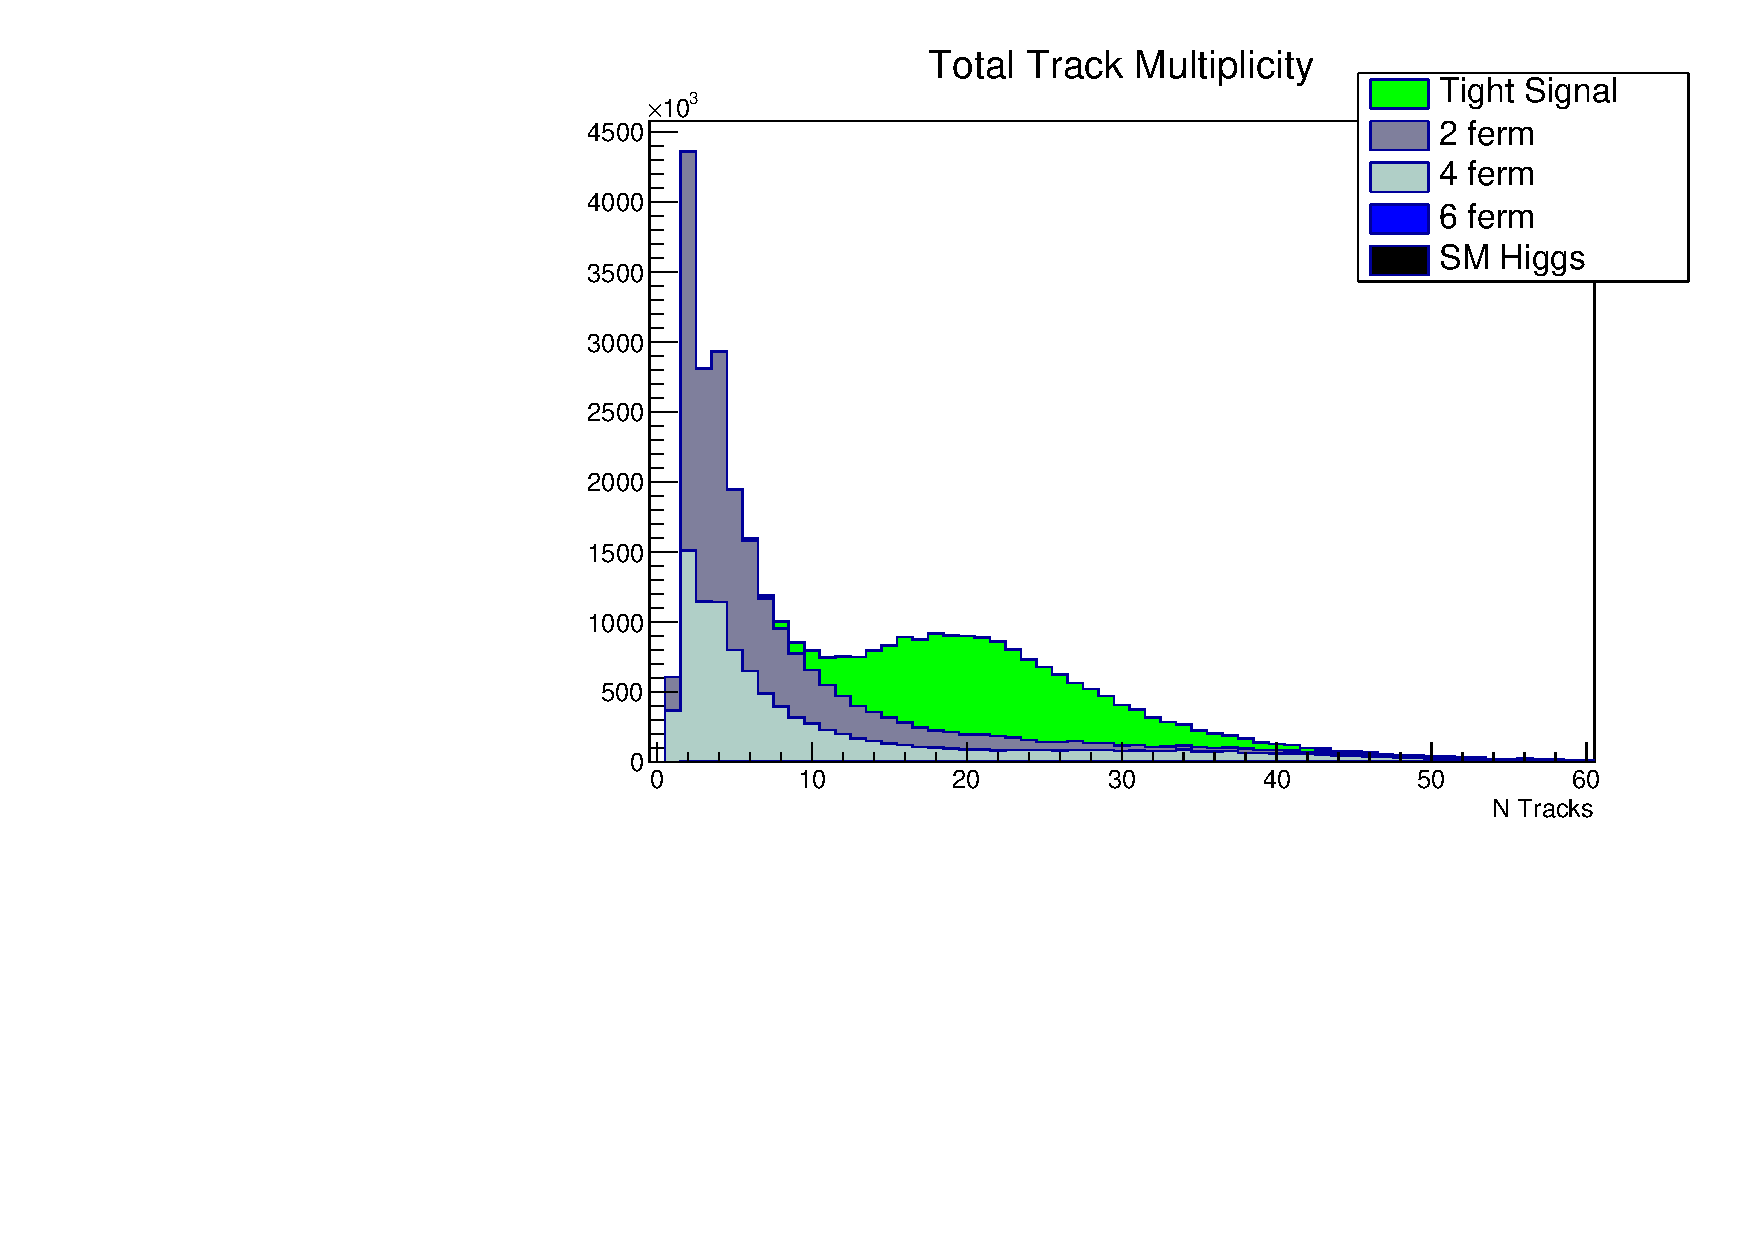
\includegraphics[width=0.9\textwidth]{ntracksHist.pdf} % second figure itself
       
     \end{minipage}\\

 \centering
    \begin{minipage}{0.49\textwidth}
        \centering
        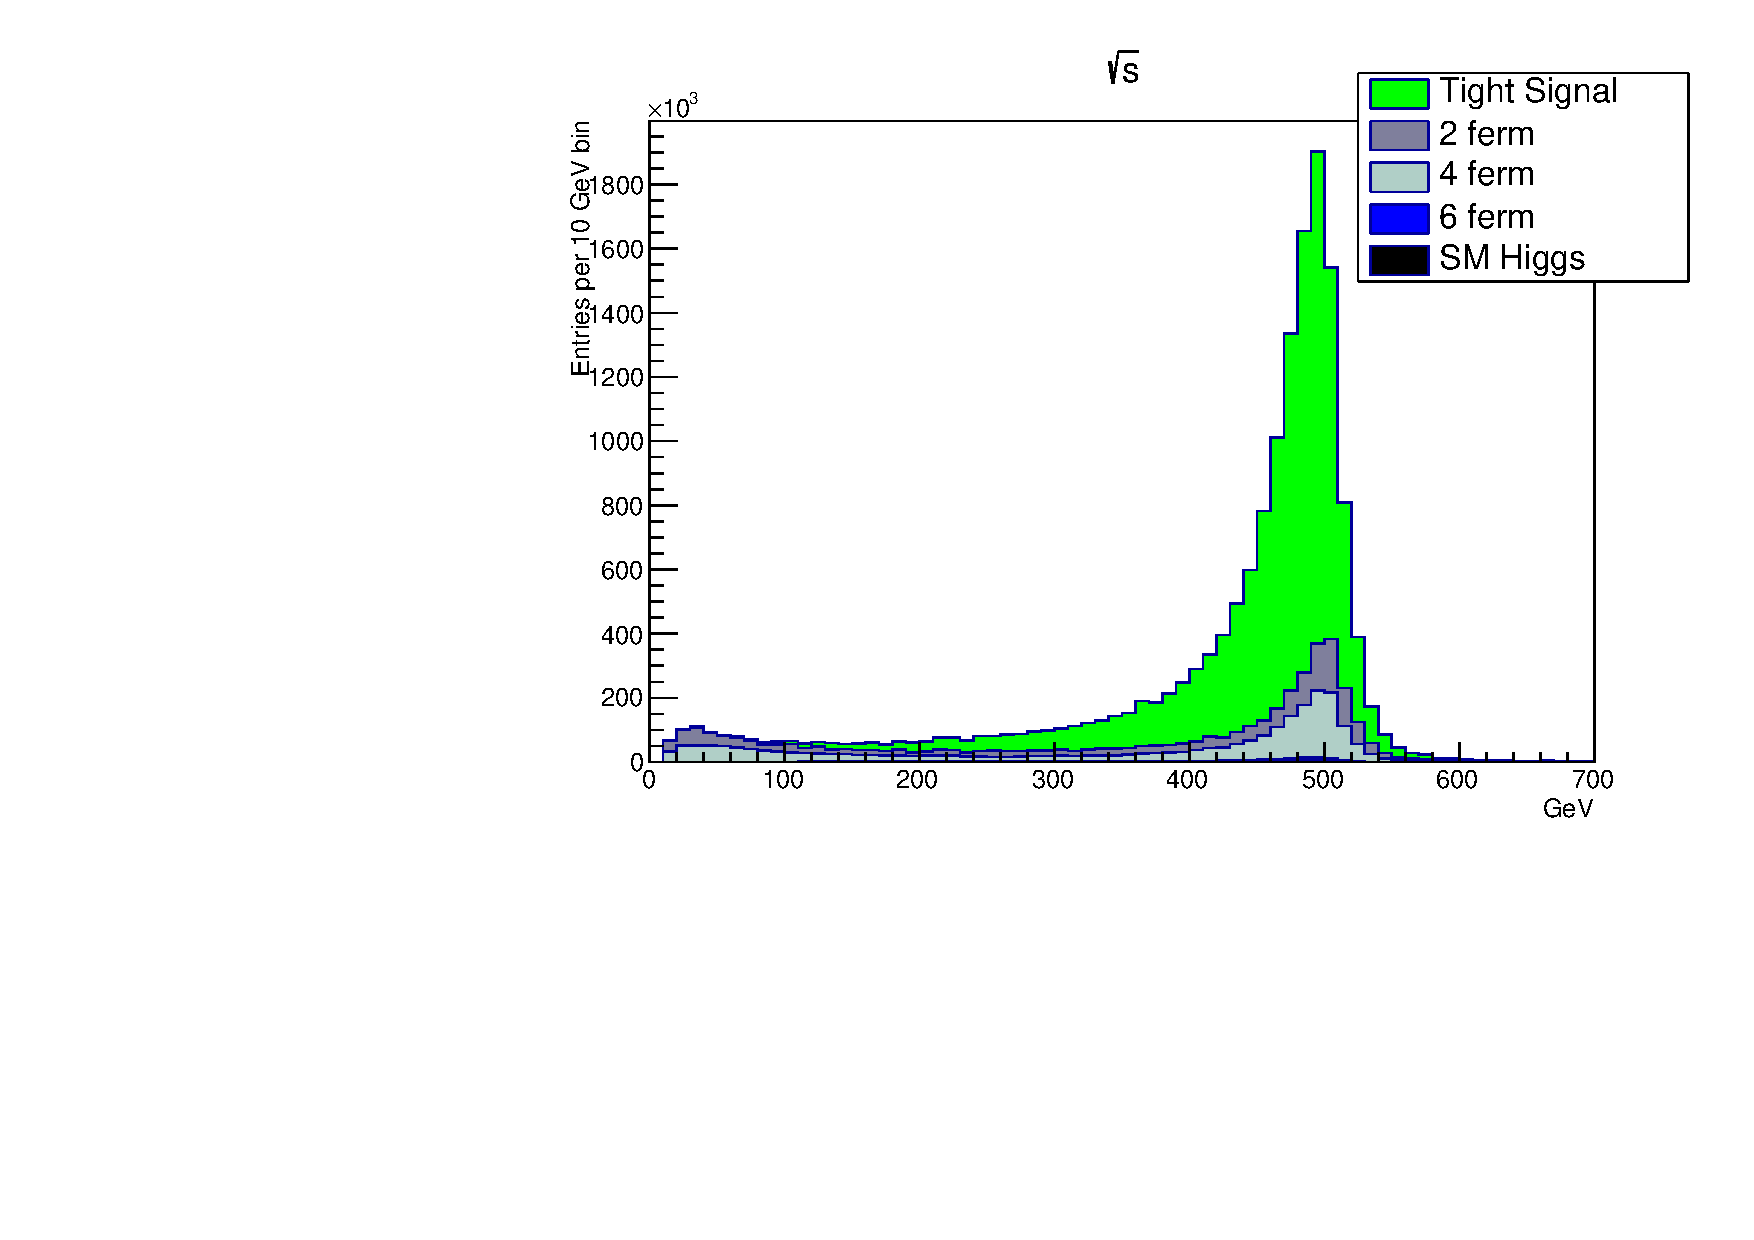
\includegraphics[width=0.9\textwidth]{EcomHist.pdf} % first figure itself
        
    \end{minipage}\hfill
    \begin{minipage}{0.49\textwidth}
        \centering
        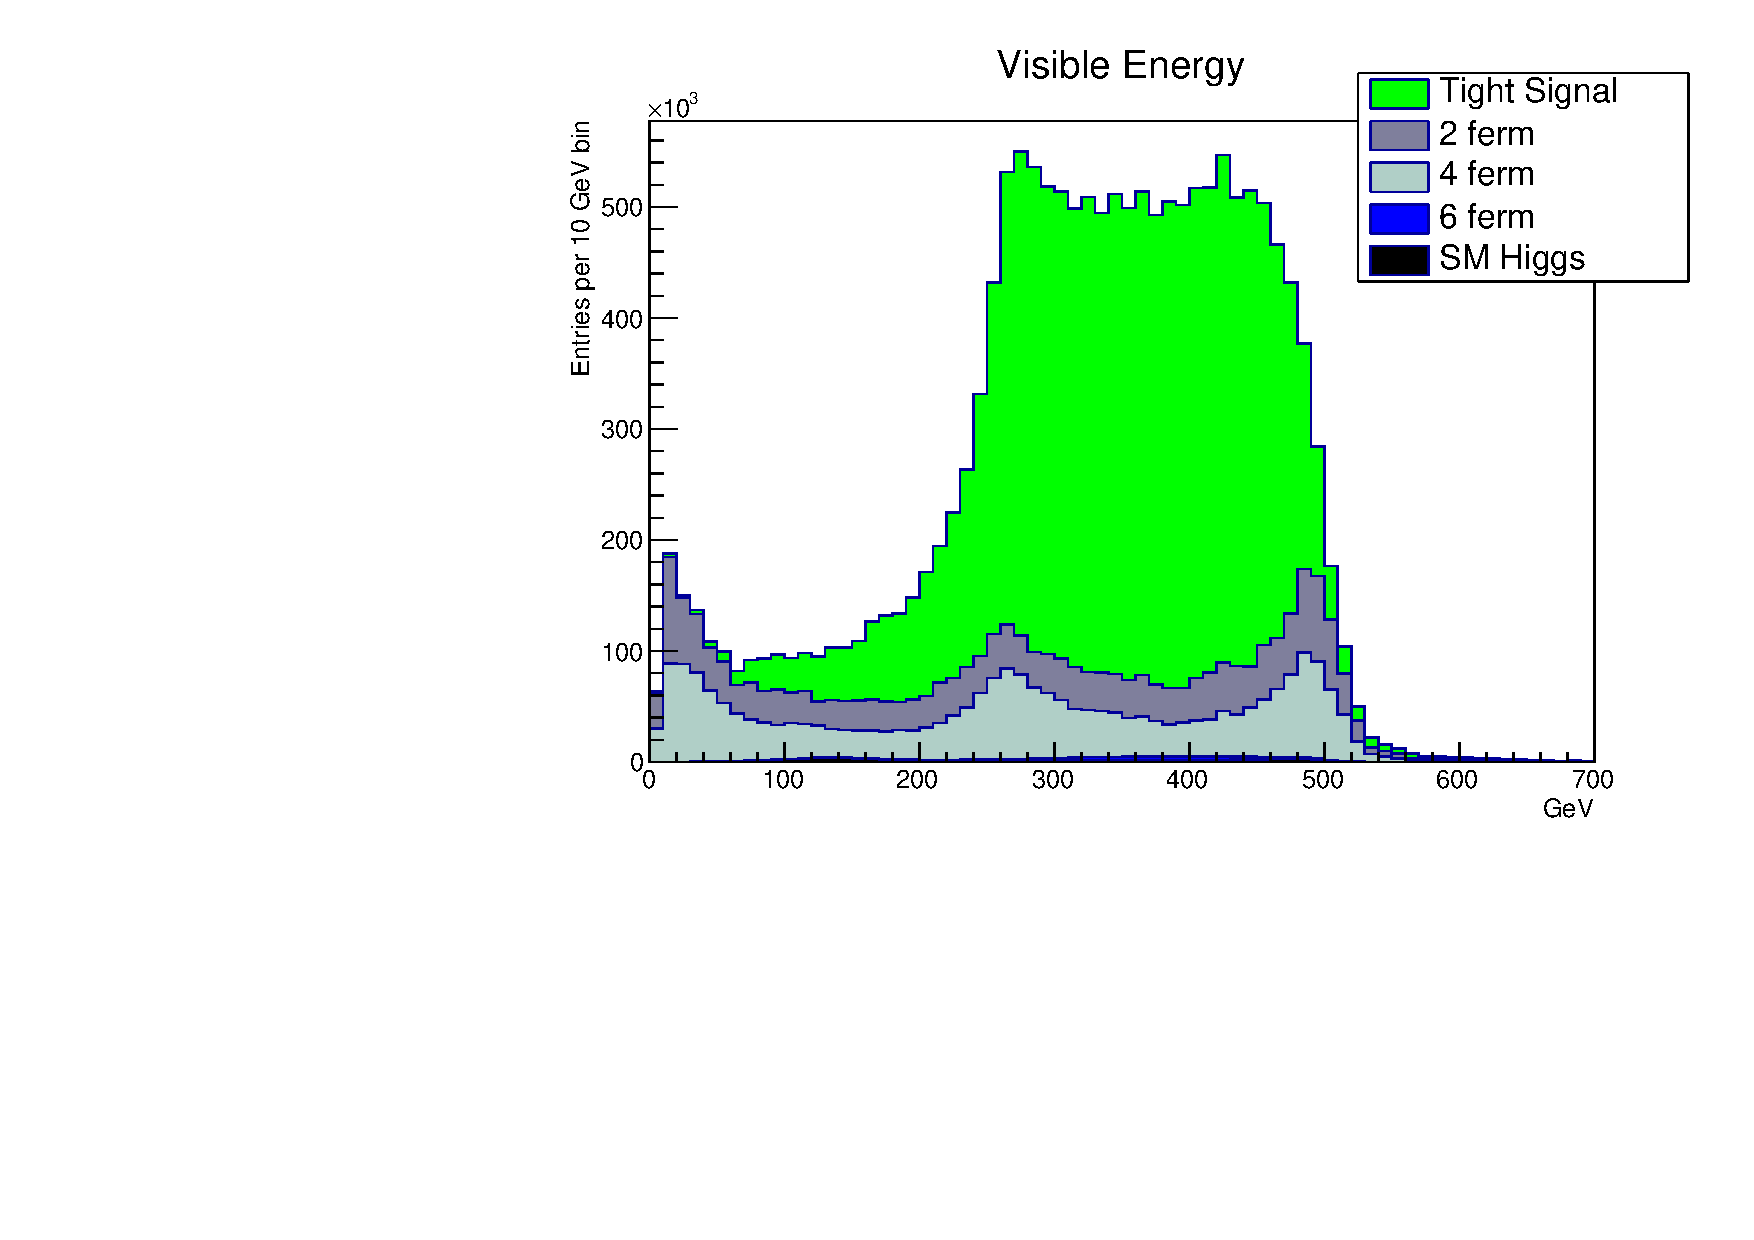
\includegraphics[width=0.9\textwidth]{EvisHist.pdf} % second figure itself
        
     \end{minipage}\\

	
 \centering
    \begin{minipage}{0.49\textwidth}
        \centering
        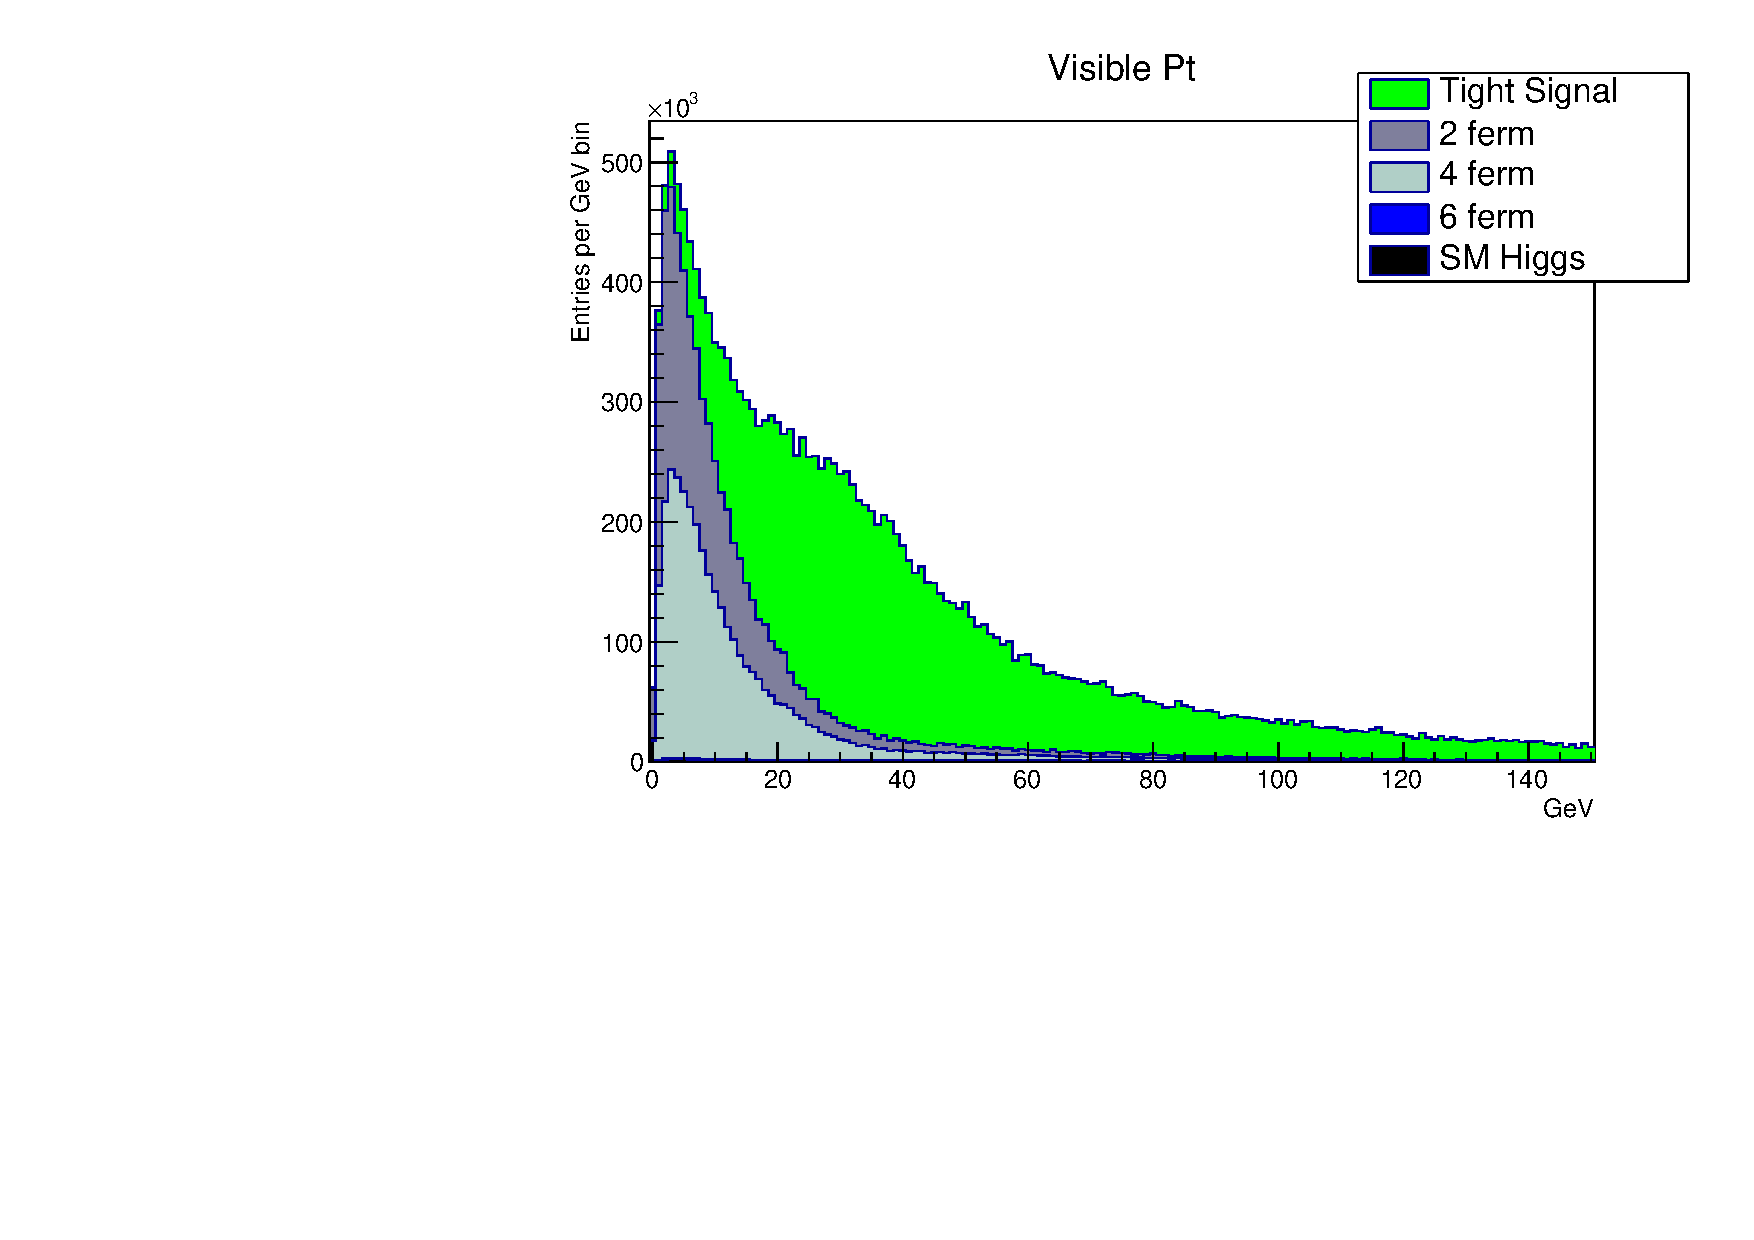
\includegraphics[width=0.9\textwidth]{PtvisHist.pdf} % first figure itself
   
    \end{minipage}\hfill
    \begin{minipage}{0.49\textwidth}
        \centering
        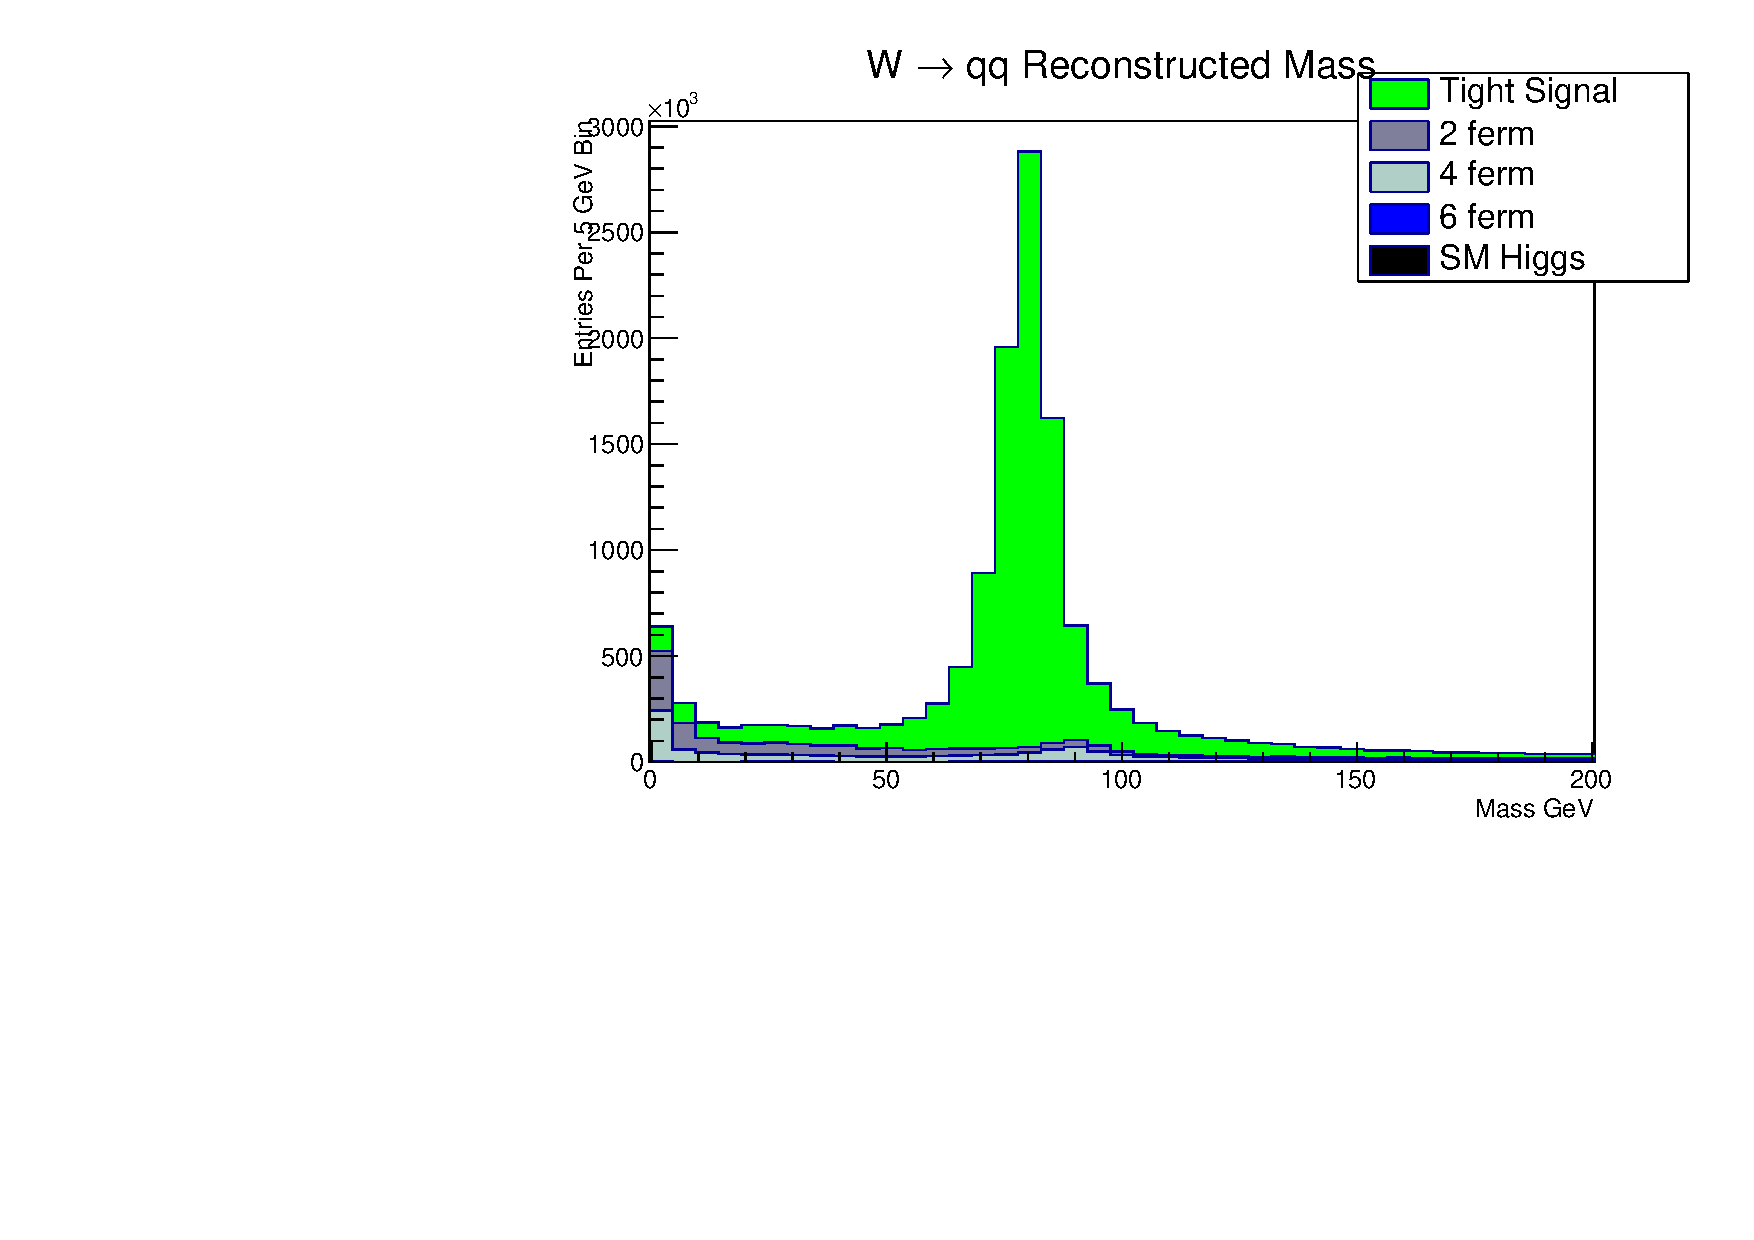
\includegraphics[width=0.9\textwidth]{mwhadHist.pdf} % second figure itself
     
     \end{minipage}\\

 \centering
    \begin{minipage}{0.49\textwidth}
        \centering
        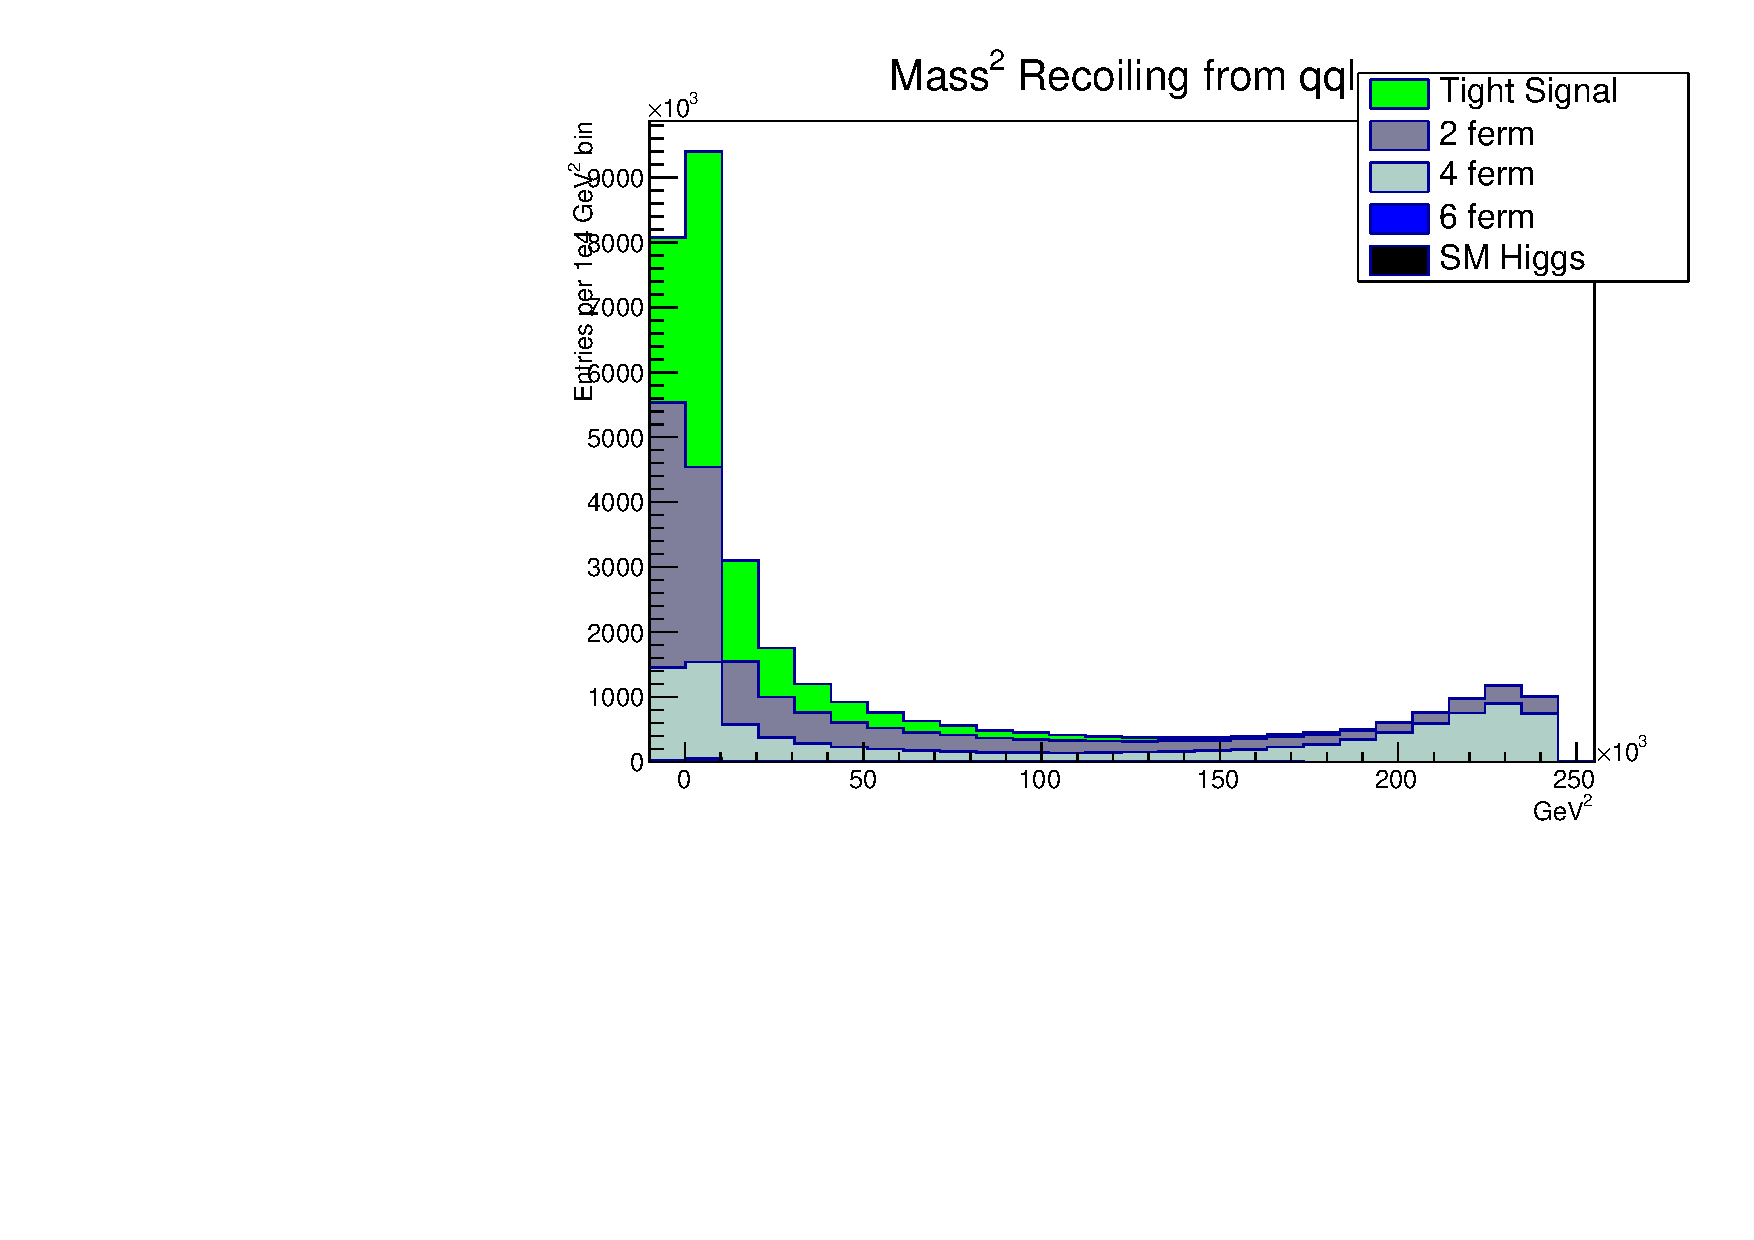
\includegraphics[width=0.9\textwidth]{vrecoilHist.pdf} % first figure itself
       
    \end{minipage}\hfill
    \begin{minipage}{0.49\textwidth}
        \centering
        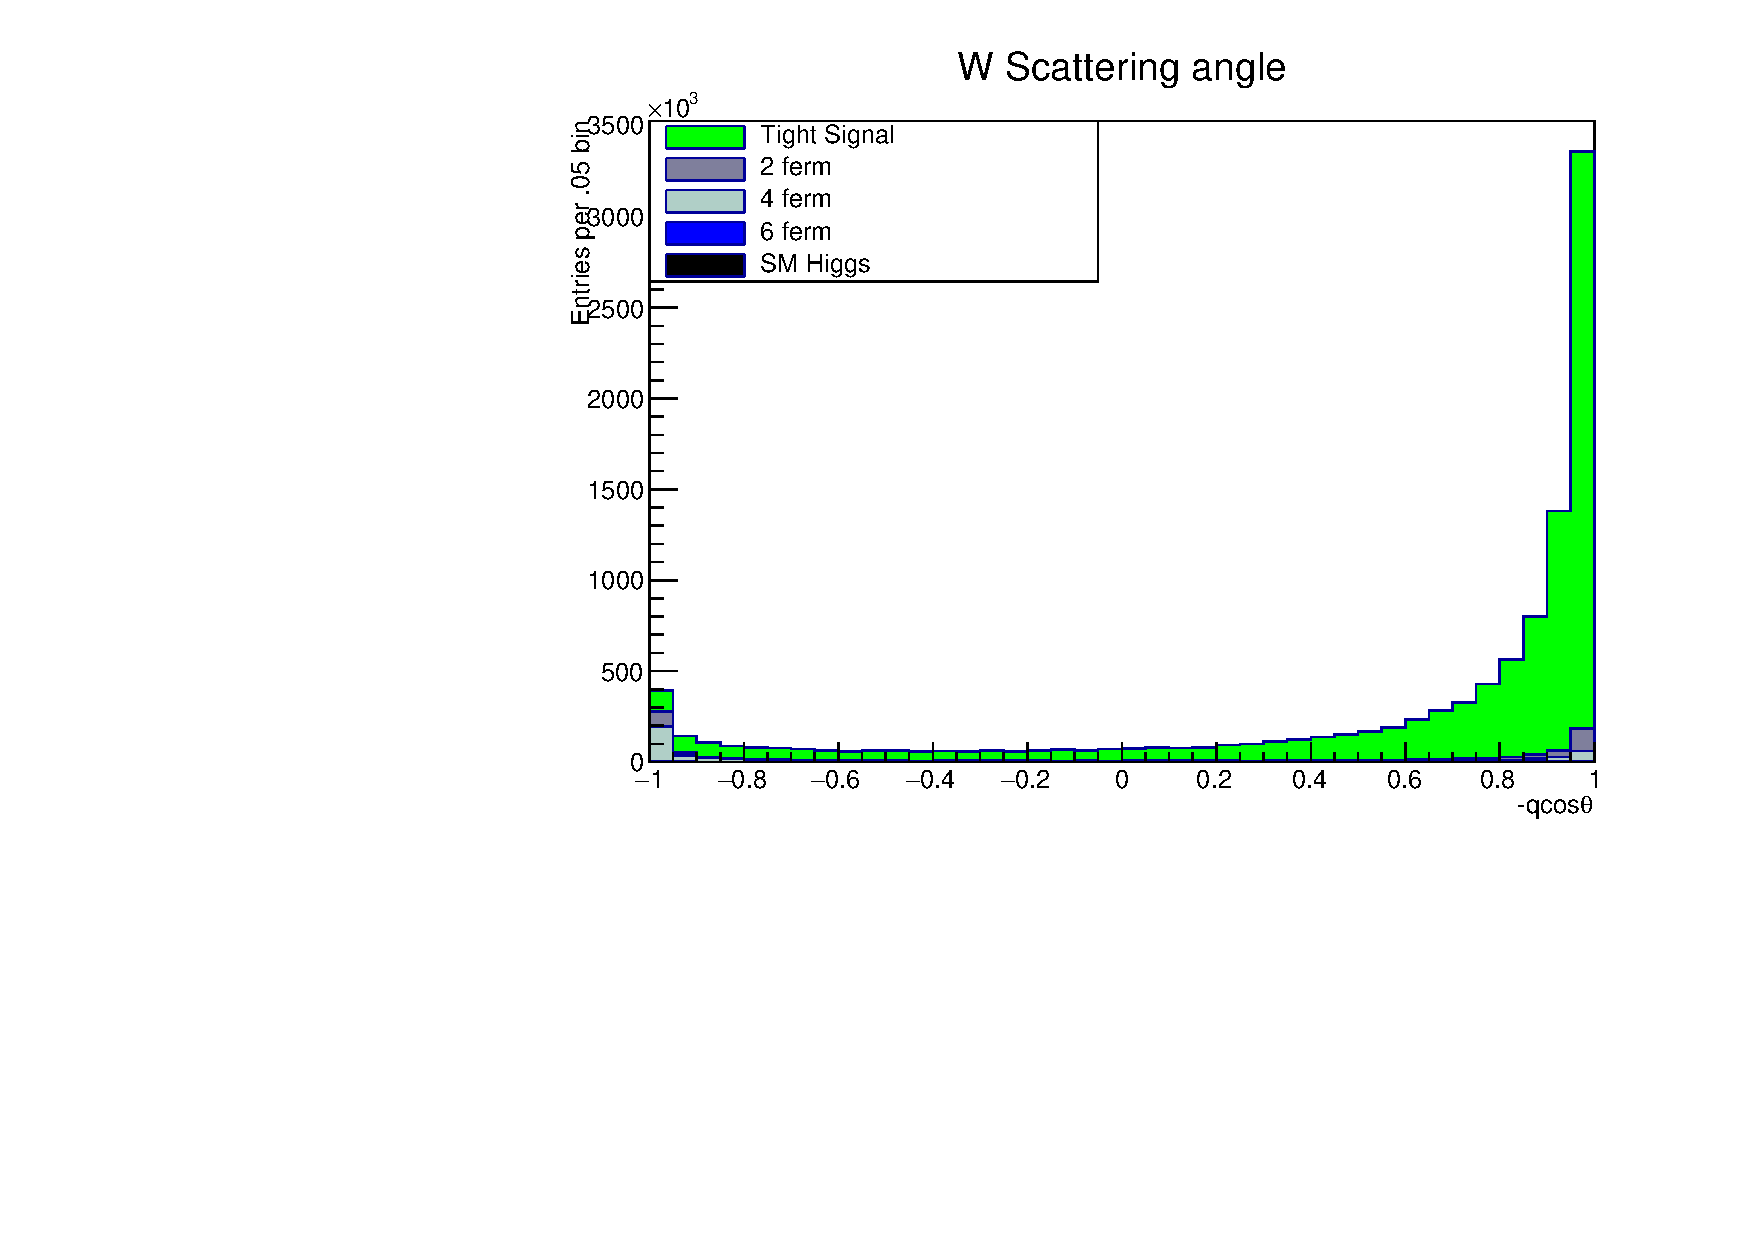
\includegraphics[width=0.9\textwidth]{qcostHist.pdf} % second figure itself
        
     \end{minipage}
          \caption{ Variables used in WW selection. Signal is comprised of the events selected with the muon cone only for all three possible final state leptons ($\mu,e,\tau$).  The beam scenario is L = 1600$\text{fb}^{-1}$ (-0.8,+0.3).}
          \label{fig:stacks1}
\end{figure}